\section{Introduction}
\label{sec:introduction}
From the Internet of Things (IoT) to the Internet of 
Everything (IoE), the 
common denominator is \emph{connectivity} driven by 
ubiquitous mobile devices. The goal of these devices and 
infrastructures is to 
build a 
cyber-physical framework that predicts and automates the 
mundane, enabling 
people to concentrate on more productive and creative things 
\cite{weldon2016future}. This digital infrastructure puts 
sensors on everything 
(animate and inanimate), links the sensors, does data 
analysis on the 
information generated by these \emph{things} to create a 
knowledge-base, makes 
predictions based on the available information and if it 
detects an anomaly, 
may take corrective, preventive or stabilizing action on the 
system. In this way, it produces a new utility 
in the form of 
time which is a positive aspect. On the downside, this 
increased connectivity 
era implies that an automated system handles both our safety 
and non-safety 
critical data and actions, and a breach in the intended 
behavior of the 
connected devices could prove catastrophic as they manage our 
daily activities 
from medicine to autonomous vehicles, avionics and power 
systems. For edge devices which are characterized by their bespoke nature and constrained compute and energy resources, this era of increased connectivity increases their vulnerability. Hence, the need to run other security and safety control modules to maintain the integrity of their operations in addition to the primary functional requirement, especially devices that manage the routines of people living with disabilities. This additional requirement 
means that these edge devices have to manage their available 
resources to satisfy both the primary objective and the 
anomaly model. While some of the devices may not require 
online anomaly monitoring due to the low-risk level 
associated with their operations, some others that perform 
critical tasks within a constrained time window require a 
constant update on the integrity of its operation. Hence, the 
need for an online anomaly model that can be integrated into 
these devices to monitor the conformity of the behavior of 
the applications installed on the devices using the 
prescribed operational standards. To optimize the impact of the anomaly framework on the performance of the device to its primary objective, we introduce a task offloading mechanism that leverages any available resources within the network created by a Wi-Fi or Ethernet hotspot. The offloading ensures that the connected devices satisfy both the demands of the main application and that of the anomaly framework. 
\par  
If the behavior of the edge devices and their 
applications are 
well-characterized, then the state transition checks espoused 
by the authors in 
\cite{sumner2013comparative,li2017locating} can be applied to 
detect the 
anomalies. However, there are two challenges associated with 
this method of 
anomaly detection in this era of data and connectivity 
explosion; 
\begin{enumerate*}[label={\alph*)},font={\bfseries}]
	\item it is daunting to define all the possible states of 
	the tuples 
	associated with a particular process running in the 
	embedded system because 
	of the increasing complexity of tasks performed by these 
	processes.
	\item the increasing complexity of the functions  
	performed by these cyber-physical embedded systems 
	demands a high level of 
	dynamism which makes the use of static state transition 
	analysis untenable.
\end{enumerate*}  
Therefore, we propose a \emph{modular, distributed} and 
\emph{scalable} 
anomaly detection framework that utilizes the temporal 
information in the system 
call execution sequences to detect anomalies. 
\par  
To facilitate the capture of long and short-term temporal 
dependencies, we use 
a stack of the Long Short-Term Memory (LSTM) 
\cite{hochreiter1997long} that learns the temporal 
relationships 
amongst the kernel events while the 
attention layer determines in small details, the impact of 
each feature in one 
another. This strategy helps to filter out the effect of the 
randomness 
prevalent in kernel events as a result of interrupts. Our 
anomaly framework uses a 
context-aware variant of the attention mechanism which does 
three functions; 
\begin{enumerate*}[label={\alph*)},font={\bfseries}]
	\item within tuples in a window under consideration, it 
	improves the target 
	tuple prediction accuracy by diminishing the effect of 
	unessential source 
	inputs for any target output.
	\item it narrows the dimension of the hidden state output 
	of the LSTM and 
	introduces flexibility in handling the size of the output 
	vector.
	\item between predictions, the attention layer controls 
	the influence of 
	the previous output on the next target by forming a 
	component of the 
	context vector that controls the alignment of the next 
	prediction.
\end{enumerate*}
And this helps to answer the \emph{why} question in the 
computation of the prediction by giving us a view of the 
\emph{features} that 
influence each output. The logic in 
our reasoning is that just like natural language, each tuple 
has different 
contexts based on usage and the effect of the present tuple $ 
\bm{V_t} $ on 
next 
prediction $ \bm{V_{t+1}} $ should be derived from a deeper 
and longer context 
than 
just the present tuple $ \bm{V_t} $ and the present attention 
vector $ \bm{Z_t} 
$ because concurrently running tasks can make the order of 
the traces complex 
to analyze. 
Therefore, in comparison with other design architectures, our 
design varies on 
how the context vector is constructed and used in both the 
attention layer and 
next target prediction. And this is one of the principal 
technical 
contributions of the work. \par
The modular design of the anomaly framework of Fig. 
\ref{fig:dataflow-model} is to allow partial or full offload 
of 
its component to a 
peer device that augments the computational capacity of the 
source device. Each monitored application has its own model 
trained using its own events. This application or 
process-focused design has the advantage of providing 
fine-grained security details in case of an anomaly, but the 
resource demand quickly escalates with an increasing number 
of applications or process running at the same time; hence 
the motivation to form an ad-hoc network as explained below. 
\par 
The motivations in creating the ad-hoc network 
are;
\begin{enumerate*}[label={\alph*)},font={\bfseries}]
	\item the devices have different behavioral patterns. 
	Some have applications that work at intervals, others 
	have applications that only respond to the environment, 
	etc. 
	This means that some of these devices have their 
	resources lying idle some of the time because of the 
	nature of the application it is running.
	\item some devices have powerful CPUs and good enough 
	memory size but as expected, they handle more 
	applications than low resource devices. Therefore, these 
	kind of devices tend to generate more traces than their 
	peers that are reactive in nature. For example, there are 
	smartwatches that are equiped with $ \bm{2GB} $ of RAM 
	today but the most common tasks of these devices is 
	notifications. 
\end{enumerate*}
Therefore, it benefits both the devices with low and high 
capacity to join the anomaly detector ad-hoc network so as to 
leverage peers' 
resources when available. Since devices with high capacity is 
more likely to have more applications that need monitoring, 
and some low capacity devices behavior tends to be bursty, it 
produces a symbiotic outcome for both types of devices with 
diverse capacities and justifies the need to form a 
network.\par

Example of the characteristics of system calls sequence is 
$\text{open} 
\longrightarrow
\text{mmap} \longrightarrow \text{read} \longrightarrow 
\text{close}$ and 
these are used as features to train the model for each 
application being monitored. Therefore, we have two problem 
statements as thus: 
\begin{enumerate*}[label={\alph*)},font={\bfseries}]
	\item given kernel events obtained during the normal 
	operation of an application or a process, 
	is it possible to create a model that uses the 
	information from the
	normal behavior of the process to detect deviant 
	behaviors in the kernel events?
	\item if yes, can we dynamically deploy this anomaly 
	model to perform online anomaly detection by leveraging a 
	pool of resources provided by an ad-hoc wireless local 
	area network?
\end{enumerate*}
To answer the questions posed above, we propose a 
\emph{modular, distributed and 
scalable anomaly detection framework} primarily targeting 
edge devices. In summary, our contributions are:
\begin{enumerate*}[label={\alph*)},font={\bfseries}]
	\item First, we present a modular deep learning anomaly 
	detection framework that uses kernel events of processes 
	to observe 
	the operation of the applications on the device.
	\item Then, we show how to leverage the modular nature of 
	the anomaly framework to create a dynamic, distributed, 
	and scalable network of nodes working together to 
	improve the security of all participating nodes. 
	\item Finally, we test the performance of the task 
	scheduling algorithm against the baseline of not joining 
	the network and show why the anomaly detector ad-hoc 
	network is a good bargain for all participating nodes in 
	terms of 
	throughput and improved security.
\end{enumerate*} \par
To ease the comprehension of the work, we have divided the 
rest of the work 
into the following sections; Section \ref{sec:related-work} 
briefly highlights 
the related work in this domain. Section \ref{sec:model} 
discusses the 
technical details of our model while Section 
\ref{sec:implementation} details our implementation 
strategies and discusses the tools we use to implement the 
framework. In Section \ref{sec:experiments/results}, we 
conduct the experiments to verify our hypothesis and discuss 
the results. Finally, we conclude the paper in Section 
\ref{sec:conclusion} with an insight into our prospective 
research directions.
\section{Related Work}
\label{sec:related-work}
According to \cite{chandola2009anomaly}, the two broad 
categories of detecting 
deviant behavior during system operation are \emph{intrusion} 
and 
\emph{anomaly} detection. While both techniques can detect 
previously seen 
anomalies, only the anomaly method monitors both known and 
unknown deviation 
from the standard performance behavior. The use of 
\emph{models} instead of 
\emph{signatures} enhances the capability of the anomaly 
method to track 
\emph{zero-day} vulnerabilities. The intrusion (signature) 
method has extensive 
details in \cite{garcia2009anomaly}. The obvious limitation 
of this 
signature-based method is that \emph{zero-day} 
vulnerabilities cannot be 
detected as it only searches for known signatures. On the 
other hand, authors 
in 
\cite{Ezeme2017,du2017deeplog,xu2009largescale,yu2016cloudseer}
 use the 
anomaly-based approach which involves the construction of a 
model to target 
both known and unknown aberrations. This model-based 
technique comes at the 
cost of doing \emph{feature extraction} from the operational 
profiles, 
\emph{processing} the extracted features to conform to the 
model input 
requirements, and finally, model design and training with the 
profile features. 
While this method provides versatility in terms of its target 
threat domain, it 
has higher false positives than the signature-based intrusion 
detection 
mechanisms.\par 
In \cite{Ezeme2017}, the authors explored the use of a vector 
space model with 
hierarchical clustering that creates a binary profile to 
determine if an 
observed profile sequences are anomalous or not. While this 
model shows an 
excellent result in the experiments used by the authors, its 
scalability is 
limited because of the enormous number of tuples it needs to 
make a decision. 
Authors of \cite{yoon2017learning} also have a vector space 
model based anomaly 
detection method which categories system processes using 
their system call 
information. This model suffers from the same scalability 
issue as that of 
\cite{Ezeme2017} because it requires a long window of 
observation before it can 
make a decision. The authors of \cite{du2017deeplog} built an 
anomaly detection 
framework called \emph{Deeplog} using two layers of LSTM 
networks and a 
workflow construction approach for each 
key in the log for diagnostics. This \emph{Deeplog} framework 
uses LSTM also, 
but there is no notion of attention layer in the framework. 
Also, the authors 
of \cite{gu2005detecting} used the statistical metric of 
entropy to implement 
an anomaly detection model for network logs but this type of 
anomaly model is 
best suited for cases where the volume of logs determine if 
an anomaly has 
occurred as obtainable in denial of service attack. In 
\cite{salem2016anomaly}, a real-time system anomaly 
detection model is 
designed using the principle of inter-arrival curves to 
detect anomalous traces 
in a log sequence. However, this inter-arrival curve-based 
model works offline 
because it requires a large number of logs before it computes 
the curves. 
Reference \cite{xu2009largescale} designed a vector space 
model to mine console 
logs for anomalies and \cite{li2017locating} used an 
optimization method of 
minimum debugging frontier sets to create a model for 
detection of 
errors/faults in software execution. In 
\cite{Ezeme2018RTCSA,ezeme2019dream}, the authors use 
the kernel event tuples to design an anomaly model based on 
the concept of the 
encoder-decoder approach. It uses an attention layer to aid 
in sequence 
reconstruction at the prediction phase. Although this 
approach is close to our 
method, we differ both in the deep learning model design and 
the entire framework implementation. 
Hence, while we introduce a load migration scheme to ensure a 
truly dynamic and 
distributed anomaly framework, \cite{Ezeme2018RTCSA} creates 
a 
monolithic anomaly 
model that places a considerable strain on embedded system 
resources, thereby 
limiting its use for online anomaly detection. Also, the 
methods 
advocated in \cite{Ezeme2018RTCSA,ezeme2019dream} 
involves the use of KNN classifier at the anomaly decision 
stage which reduces the applicability of such approach in a 
near real-time application. Also, the authors of 
\cite{chawla2018host} did a host-based anomaly detection 
using a combination of CNN/RNN where the CNN acts as a filter 
and the RNN helps in remembering contexts over a log span of 
sequences. Furthermore, the authors of \cite{serpen2018host} 
used a mixture of PCA algorithm and KNN classifier to perform 
host-based anomaly detection on system traces. As expected of 
many clustering-based processes, 
\cite{serpen2018host,Ezeme2017} suffer from being unusable for online analysis. In \cite{al2019anomaly}, a 
graph-based anomaly detection scheme based on system calls 
was developed. While this is lightweight and can run online, 
it cannot handle a previously unseen type of sequences 
without rebuilding the graph. Finally, 
\cite{marteau2018sequence} use the concept of sequence 
covering to develop an anomaly detection model using system 
calls as the sequence of interest.


\section{Proposed Approach}
\label{sec:model}
\subsection{Definition of Terms and Assumptions}
\label{subsec:system}
\begin{figure}[!t]
	\centering
	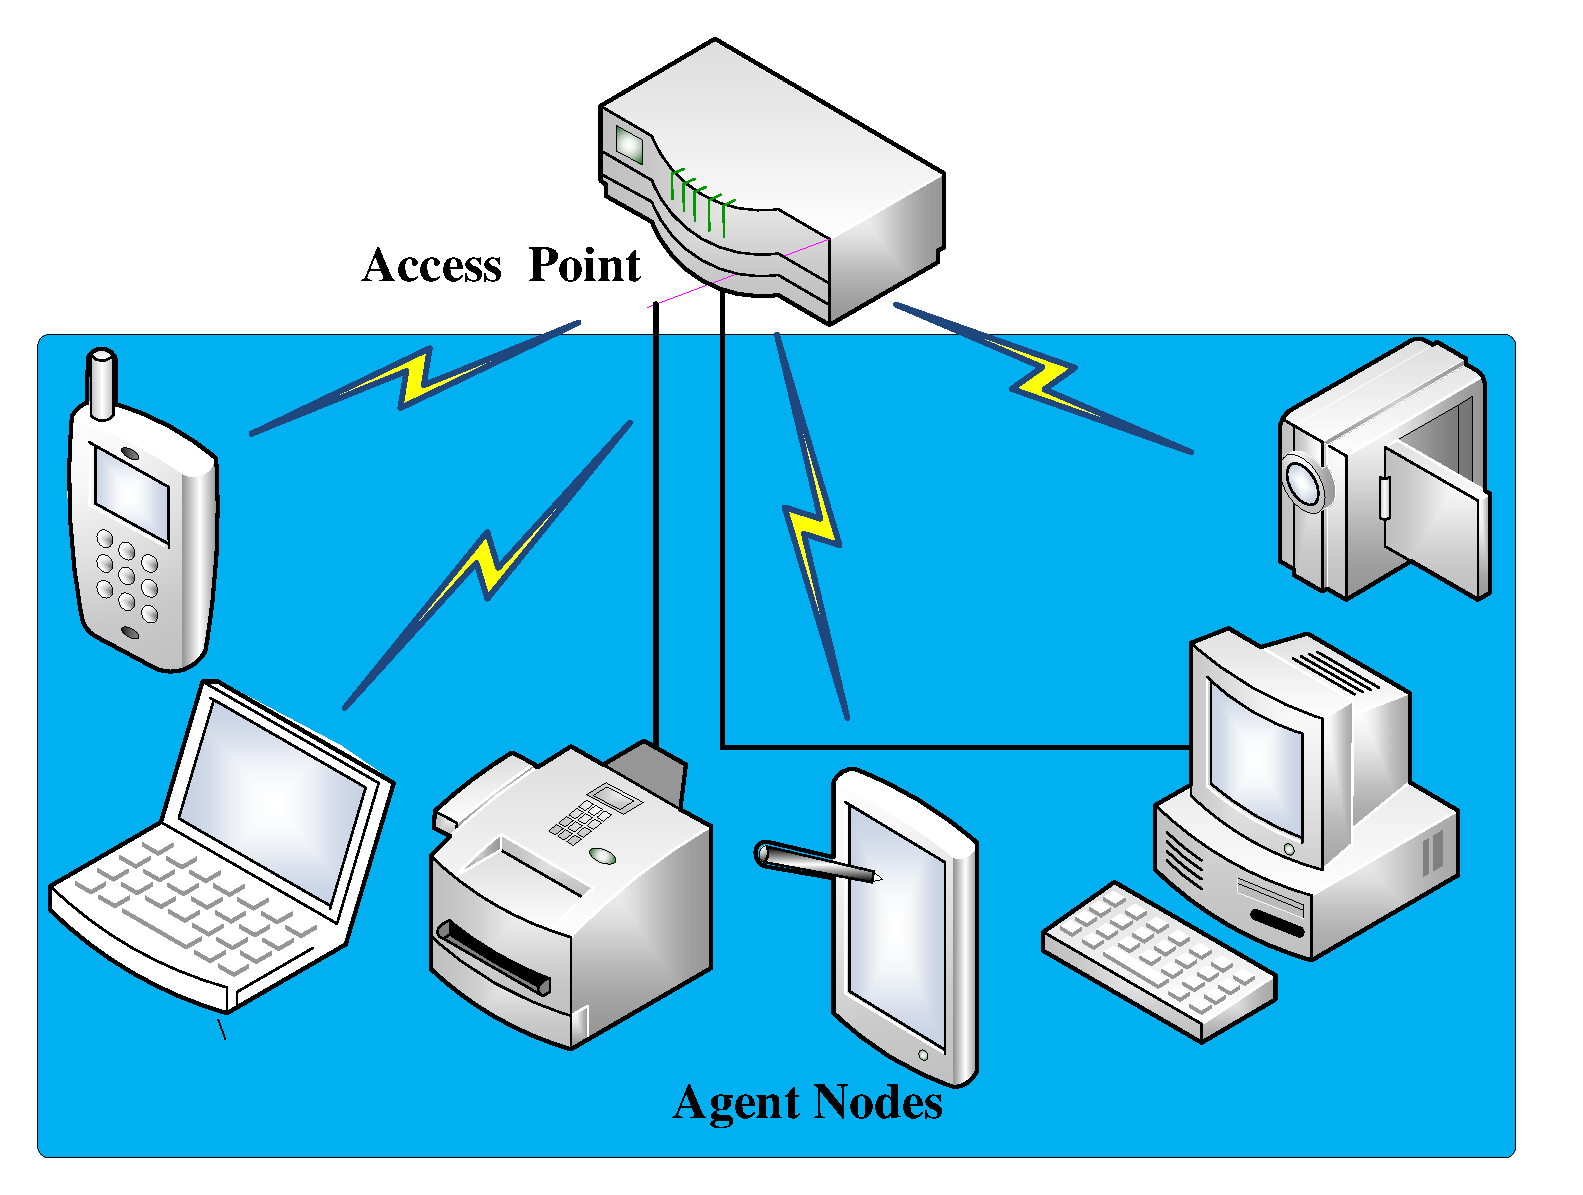
\includegraphics[width=0.49\textwidth, 
	height=7cm]{dade} 
	\caption{Network Design with Diverse Nodes}
	\label{fig:system-architecture}
\end{figure}
The network consists of \emph{nodes} of diverse 
capabilities and behavior and an \emph{access point} like a 
router. While the node can access the internet and 
other external services via the access point, our 
network does not include nodes in the cloud or outside the 
local network. Our design brings online capability to a node  
which may or may not accommodate the extra strain on 
system resources introduced by doing anomaly detection on 
applications in the node. While the
cloud boasts of unlimited resources, latency constraints and 
the fact that some of the nodes are mobile restricts our 
design to a local network of nodes. On the positive 
side, the proximity constraints provided by the access point 
device ensures that we have an idea of the worst latency 
conditions and the nodes can easily adapt their 
applications according to the prevailing local conditions. As 
the 
network condition readily available when the node  
connects to the access point, the nodes can adaptively 
export the anomaly application wholly or partially to other 
peers in the network by running its \emph{task manager} 
algorithm that is embedded in the application. Overall, the  
network aims to optimize the processing time of tasks 
and reduce the number of tasks dropped for exceeding the 
response time constraint. \par
Therefore, the application aims to address the question of 
which part of the anomaly framework should run locally or on 
a peer to reduce processing time. In making this decision, 
the capacity of the peers, round trip time to peers, number 
of tasks on peers, energy level of peers, etc are taken into 
consideration in the task management algorithm. Hence, there 
is a competition between the local resources and the 
transmission medium. Before we introduce the model 
parameters, we define 
the following behavior of the ad-hoc network:
\begin{itemize}
	\item every node that generates a task
	also acts as a sink for the task whether it was executed 
	locally or in another peer.
	\item as with all wireless or wired local 
	networks, every traffic passes through the access 
	point. Hence, the capacity of the network is limited 
	by the capacity of the access point node. Bluetooth and 
	other peer-to-peer technologies that do not support 
	multi-input, multi-output paradigm are not considered 
	because our application is multi-threaded.
	\item in the dataflow model of Fig. 
	\ref{fig:dataflow-model}, the application has been split 
	into parts with designations of possible points of 
	execution. If a task is offloaded at the 
	\emph{predictor} stage, 
	then the peer that executes the task determines where 
	the 
	detector runs but the result must go back to the 
	source 
	of the task. 
	\item movement of peers within the network does not 
	alter the network topology.
	\item nodes do not route traffic. 
	Therefore, the ad-hoc network is a one-hop network, and 
	the one-hop is the access point node. 
\end{itemize}

\begin{figure}[!t]
	\centering
	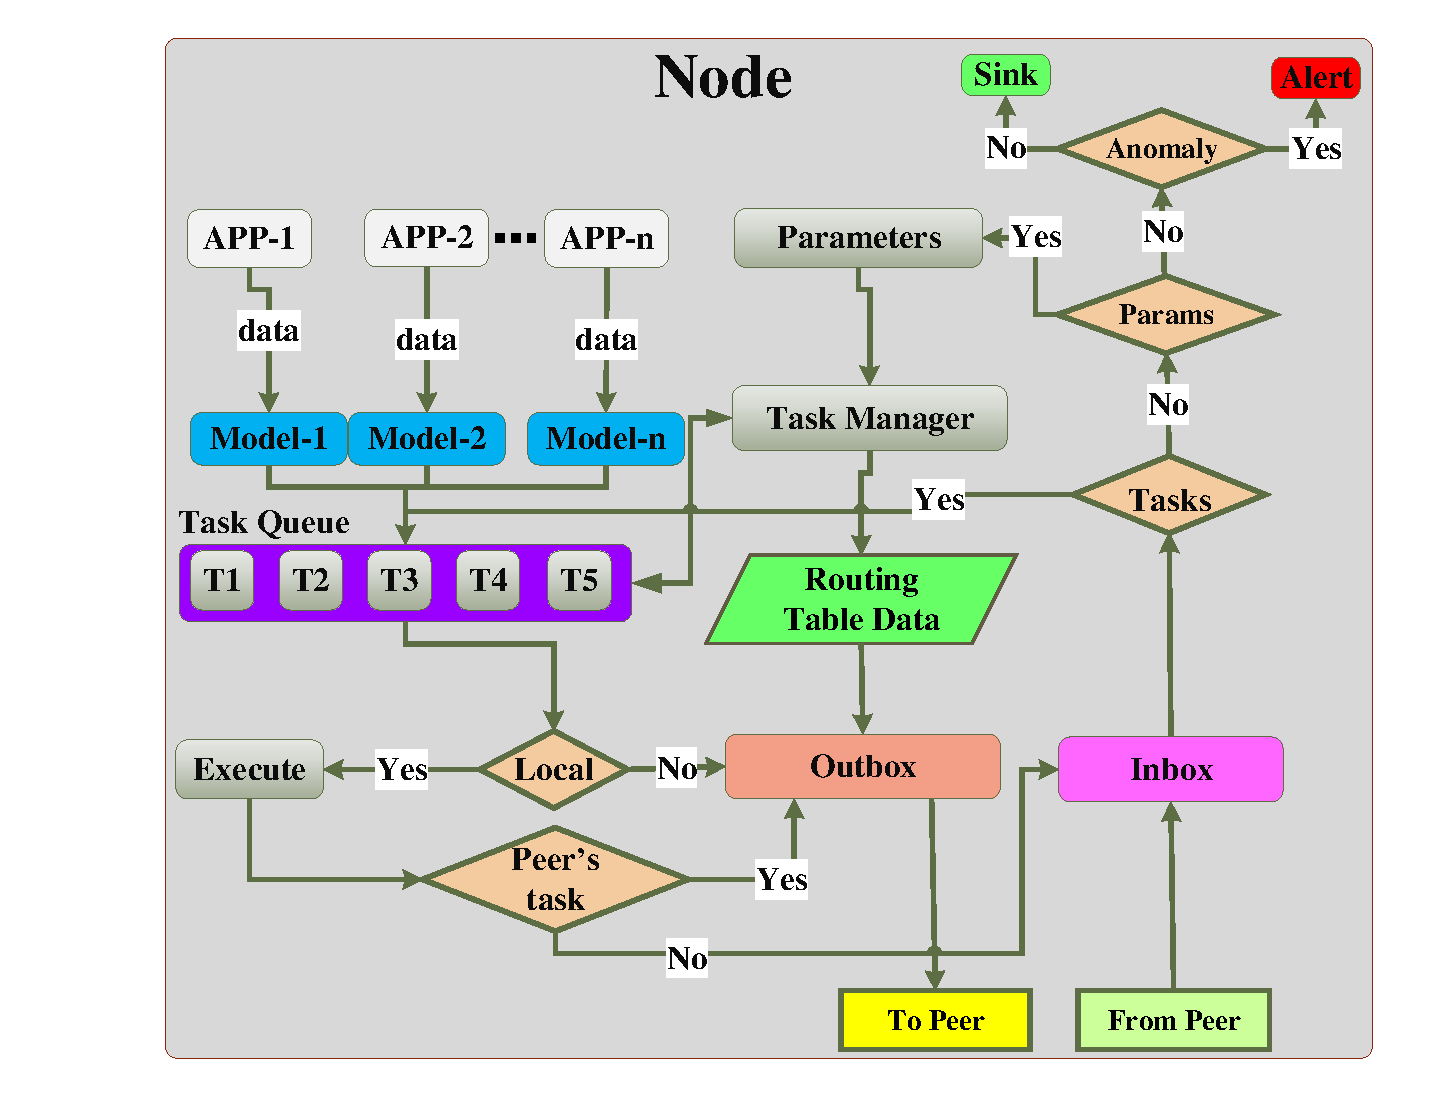
\includegraphics[width=0.49\textwidth, 
	height=7cm]{agent} 
	\caption{Implementation Diagram of the Anomaly Detection
	Application in a Node}
	\label{fig:agent}
\end{figure}
\subsection{Problem Statement}
\label{subsec:problem-formulation}
\begin{figure}[!t]
	\centering
	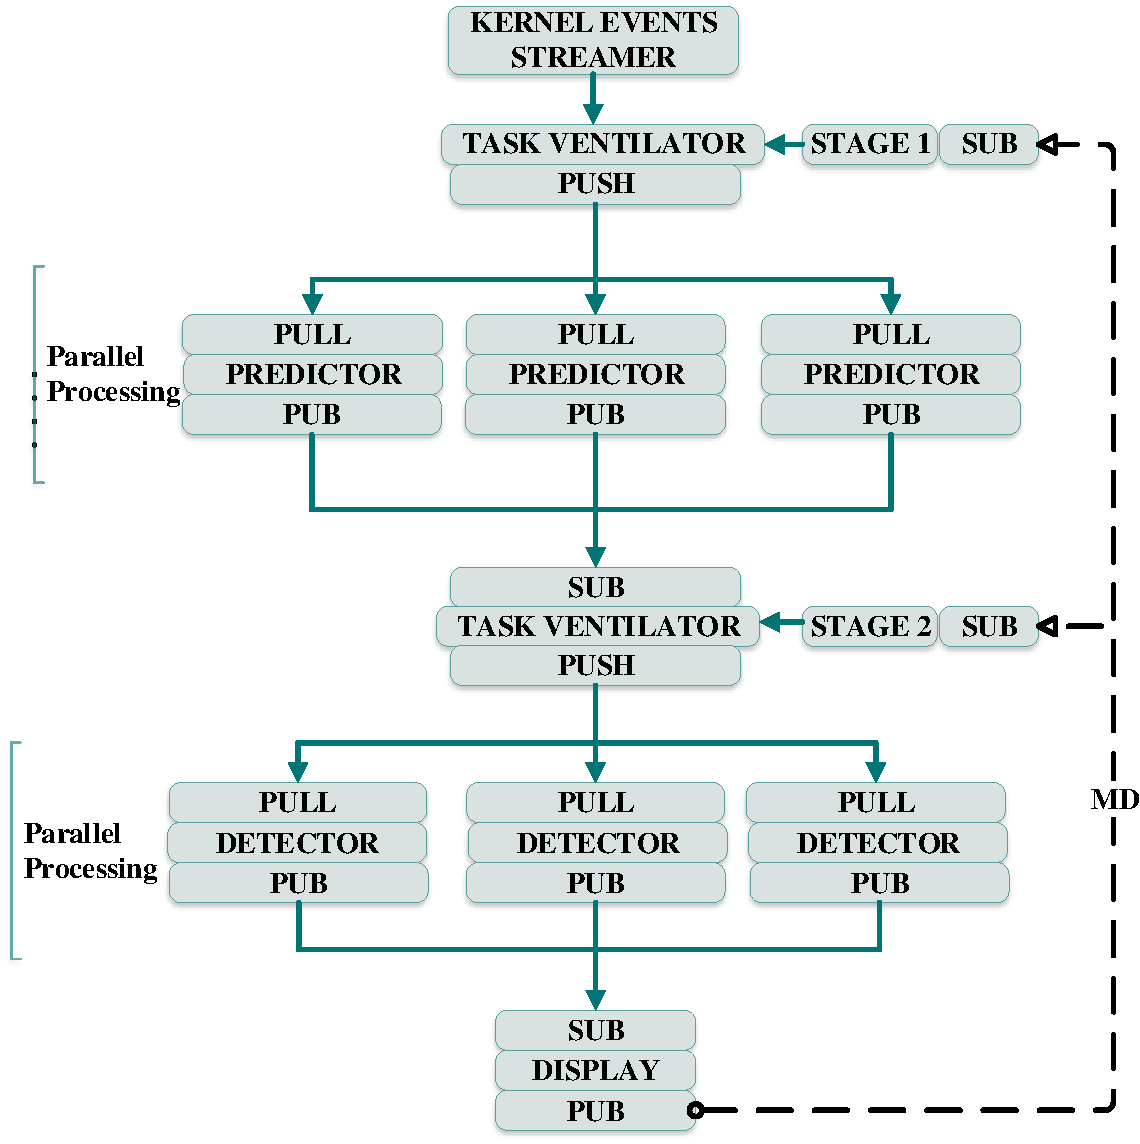
\includegraphics[scale=0.45]{decomposed-model}
	\caption{Dataflow Model of the Anomaly 
		Detection Framework}
	\label{fig:dataflow-model}
\end{figure}
We model the execution flow of Fig. \ref{fig:dataflow-model} 
with a directed acyclic graph (DAG) $ \bm{G=(V,E,s_j)} 
$ made up of a set of $ \bm{v} $ task segments $ {
\bm{V=\{v_j|1\leq j\leq v\}}} $, a set of $ \bm{e} $ edges or 
arcs 
$ \bm{E=\{(j,k)|j,k \in V\}} $, and a set of instruction 
counter tag $ \bm{s_v} $ attached to every task segment 
identifying the number of CPU instructions needed to execute 
the task $ \bm{v} $. The task segments enjoy the benefit of 
parallelism provided via threads and the number of threads 
that can be created on a particular device is a function of 
the device resources spared for anomaly detection after the 
main application has taken its own required resources. If a 
task, $ \bm{v} $ is to be offloaded to a peer, \emph{ZeroMQ} 
sockets are used to transfer data between peers in the 
network. Hence, the ports in Fig. \ref{fig:dataflow-model} 
are attached to \emph{ZeroMQ} sockets. We chose \emph{ZeroMQ} 
in our design because sockets can disappear and reappear 
without needing to restart the pair. Hence, we can scale up 
or down the number of concurrent \emph{predictors} or 
\emph{detectors} at runtime so as to optimize the latency 
reduction. Therefore, with the knowledge of the properties of 
the graph $ \bm{G} $, the CPU capacity, $ \bm{\alpha_k} $ of 
the node $ \bm{k} $, the 
fraction of the CPU for anomaly detection, $ \bm{\beta_k} $ 
and 
the capacity of the wireless channels, $ \bm{B} $, the 
problem becomes finding the minimum task finish time of $ 
\bm{v} $ task segments, ${ \bm{V=\{v_j|1\leq j \leq v\}}} $ 
given a $ \bm{n} $ set of peer nodes ${ \bm{N=\{n_k|1 \leq k 
\leq n\}}} $. To get the peers parameters required for 
computing the task finish time algorithm, the nodes 
rely on the access point node to reduce the congestion 
occasioned by parameter updates. If each peer has to query 
each other for updates, then each node requires $ \bm{2 
\times n} $ messages to get a view of the network. And 
considering that all these messages pass through the access 
point, ${ \bm{(2\times n\times n)}} $ messages will have to 
pass 
through the wireless channel $ \bm{B} $ for parameter update 
alone. We consider this a significant strain on the network 
considering that these updates are frequent. Hence, our 
decision to use the access point node for parameter update 
where a broadcast signal is used to query the peers and send 
parameter update. So, parameter update in this 
instance only requires $ {\bm{((2\times n) + n)}} $ messages. 
\par 
Therefore, given the instruction count, $ \bm{s_j} $ of a 
task 
segment, and CPU resource of the node $ \bm{\beta_k 
\times \alpha_k} $, the compute time of task segments, ${ 
\bm{V=\{v_j|1\leq j \leq v\}}} $ in a given node, $ \bm{k} $ 
is given in \eqref{eq:t-local}.
\begin{equation}
	\bm{t_{j}=\frac{m_j\times 
	s_j}{\beta\times\alpha}\sum_{j\in 
	V}m_j}
	\label{eq:t-local}
\end{equation}
In \eqref{eq:t-local}, $ \bm{j} $ denotes the 
\emph{predictors} and \emph{detectors} of Fig. 
\ref{fig:dataflow-model}. If the size of the task to be 
transferred to another peer via the edge, $ \bm{e_{j,k}} $ is 
$ \bm{x_{j,k}} $, then the latency is computed in 
\eqref{eq:latency}.

\begin{equation}
\begin{split}
\bm{t_{(j,k)}} &= \bm{\min_{(j,k\in E)}( 2 
\times\frac{x_{j,k}\times|m_j-m_k|}{e_{j,k}}}\\
	&\bm{+\frac{s_j\times|m_j-m_k|}{\beta\times\alpha}\sum_{j\in
		V}m_j)}
\label{eq:latency}
\end{split}
\end{equation}
From \eqref{eq:t-local} and \eqref{eq:latency}, we derive the 
cost of processing a task as given in \eqref{eq:t-task} where 
$ \bm{m_k=1} $ and $ \bm{m_j \in \{0,1\}} $. Since all the 
peers share the same wireless bandwidth, then $ 
{\bm{\sum_{(j,k\in E)}e_{j,k}|m_j-m_k|=B}} $ and $ 
{\bm{e_{j,k}>0}} $ in \eqref{eq:latency}. Simplifying 
\eqref{eq:latency} further, the cost of procesing a task in a 
peer node becomes \eqref{eq:latency-2}
\begin{equation}
\begin{split}
\bm{t_{(j,k)}} &= \bm{\min_{(j,k\in E)}( 2 
	\times |m_j-m_k|\times(\frac{x_{j,k}}{e_{j,k}}}\\
&\bm{+\frac{s_j}{\beta\times\alpha}\sum_{j\in
		V}m_j))}
\label{eq:latency-2}
\end{split}
\end{equation}

Now, given tasks with latency requirements, $ \bm{t_{max}} $, 
the problem reduces to minimizing \eqref{eq:t-task} such that 
${ \bm{t_{T_p}^j\leq t_{max}^j, \; \forall j \in V }} $. 
Finally, this minimization algorithm is solved by each 
node independently with the help of the network information 
supplied by the access point node.
\begin{equation}
\bm{t_{T_p} = t_{j} + t_{(j,k)} } 
\label{eq:t-task}
\end{equation}
\subsection{Nodes (Devices)}
\subsubsection{Task Generation}
\label{subsec:task-generation}
The nodes of Fig. \ref{fig:agent} have 
system resources of different capacities and run diverse 
types of applications. However, while some of the 
applications tolerate delay, some others are time-sensitive. 
Hence, the size of the data that the processes $ 
\bm{\{P_1,P_2,...,P_n\}} $ of 
Fig. \ref{fig:agent} emits vary in size and time sensitivity. 
When kernel events of a process $ \bm{P} $ is fed to the 
model of Fig. \ref{fig:agent} as data, a \emph{task} $ 
\bm{T_{p}} $ is created and transferred to the task queue. To 
aid in task management and routing, each $ \bm{T_p} $ has as 
properties; \emph{data, task-type, task-uuid, 
	task-owner-name, task-size}, and the 
\emph{task-creation-time}. The 
\emph{task-type} determines the stage of the processing 
(predictor or detector) while \emph{task-uuid} identifies the 
source node for routing back results if the task is 
processed in a peer. The size of the task of a process, $ 
\bm{P} $ in bytes is denoted 
as $ \bm{d_p} $ while the $ \bm{s_{p}} $ is the number of CPU 
instruction 
cycle 
needed for the task, $ \bm{T_p} $'s execution. We assume a 
uniform $ 
\bm{d_p} $ for each $ \bm{T_p} $ of a unique $ \bm{P} $ since 
the input data is structured with a known dimension.
\par
Also, tasks can come from peers that have determined that it 
is cheaper (in terms of time) for their tasks to be executed 
in this node as shown in Fig. \ref{fig:agent}.  
\subsubsection{Task Manager}
The task manager does the cost estimation which determines 
where a task is executed taking into account the frequency of 
task generation (both internal and external generation), the 
nodes profile and the parameters supplied by the access 
point node. Equation \eqref{eq:latency} represents the 
latency of executing task segments in a peers node and 
this information is provided by the access point node which 
we have designed to have a complete view of the network. 
Since \eqref{eq:latency-2} is the latency of executing a task 
segment in a peer, \eqref{eq:t-task} can be modified to 
become \eqref{eq:t-task-2} which gives the end-to-end latency 
of a task. Also, because \eqref{eq:t-task-2} is not trivial 
to compute, we use the experimental value $ 
\bm{\text{latency}} $ obtained from the network profile 
parameters (which includes the delay, processing time, queue 
size and node CPU load information) supplied by each node to 
the access point node.
\begin{equation}
	\bm{t_{T_p}= t_j + \text{latency} }
	\label{eq:t-task-2}
\end{equation}
Since node mobility in and out of the network is 
common, and some tasks can be bursty, the task manager keeps 
a routing table which is updated each time the access point 
node sends the network parameters to avoid sending tasks to a 
stale node. The table maintains a cyclic ascending 
latency times from active peer nodes as well as their 
\emph{uuid}.
\subsubsection{Handle Task}
The task execution and offloading is determined by the 
information computed by the task manager which annotates the 
task segments with the point of execution. If a task segment 
is marked to executed locally, the \emph{execute} module is 
called, otherwise, it sends the task to the \emph{outbox} 
module which uses the routing table information to retrieve 
the peer node \emph{uuid} and the task is dispatched. If the 
local execution happened on a task, the \emph{task-uuid} is 
compared with the nodes \emph{uuid} and if the 
\emph{uuid} match, the execution result is sent to the 
nodes inbox, else that \emph{task-uuid} is used to route the 
task result back to the node that created the task.
\subsubsection{Inbox}
The \emph{inbox} module receives \emph{tasks, results}, and 
parameter \emph{query/update} locally, from peers 
and access point node, and makes the necessary check using 
the 
received data properties to take appropriate action as 
outlined in Fig. \ref{fig:agent}. 
\subsection{Access Point Node}
\begin{figure}[!t]
	\centering
	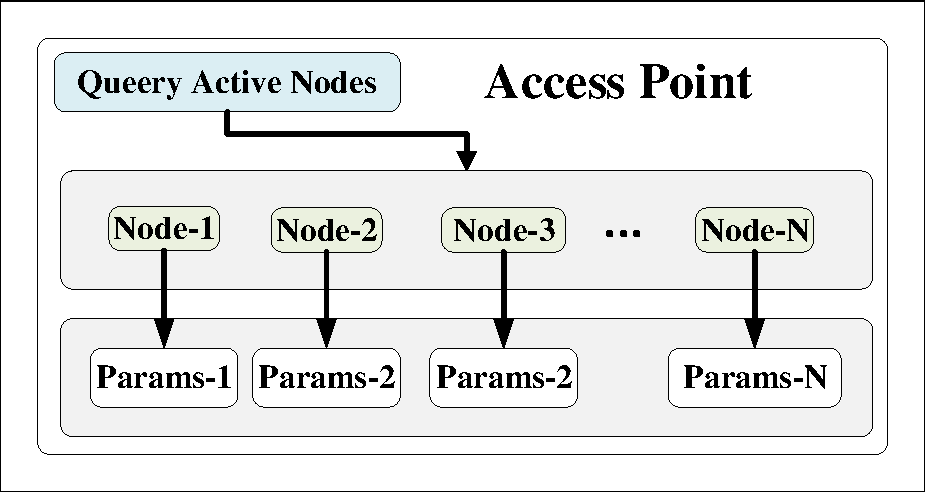
\includegraphics[width=0.49\textwidth, 
	height=5cm]{accesspoint} 
	\caption{Access Point Node}
	\label{fig:access-point}
\end{figure}
Our access point node performs two functions: parameter 
\emph{query} and \emph{update} using broadcast messages. As 
we explained in Section \ref{subsec:problem-formulation}, 
this design reduces the number of messages required for 
update by more than $ \bm{1/3} $. We are aware that this 
makes the access point a single point of failure but since it 
is central to the network formation in the first place, we 
know that the exit of the access point node terminates the 
network irrespective of whether we use it for parameter 
update or not since the Wi-Fi technology is provided by the 
access point.
\section{Implementation}
\label{sec:implementation}
To ensure an easy comprehension of the concepts discussed in 
this section, we start by describing the deep learning 
framework which is at the core of the anomaly detection 
framework. A high-level architecture of our framework is 
depicted in Fig. 
\ref{fig:rnn-model}. The 
high-level 
overview depicts a stream of kernel events traces from an 
application or a process continuously being injected into the 
anomaly framework.
We feed the streams to the deep learning models via the 
\emph{feature 
	processor} module. 

\subsection{Feature Processor}
The kernel event features of interest are the 
\emph{timestamp}, and the \emph{system call ID}. To ensure a 
deterministic 
outcome with respect to time, we use the 
CPU cycle count. In a given process or application being 
observed, given \emph{timestamp} 
as $\mathbf{t} $, and system call string name as $ \mathbf{k} 
$, we process these properties to 
yield a multi-input feature space that we feed to our models. 
These actions are captured in the \emph{Feature Processor} 
module of Fig. \ref{fig:rnn-model}. Equation 
\eqref{eq:beta} defines the processing of the time stamp to 
yield the CPU cycle count which we feed as one of the inputs 
to the model.

\begin{equation}
\bm{\mathbb{\beta}}:\left(\mathbf{t}_i,\mathbf{t}_{i+1}\right)
\longmapsto 
\mathbf{t}_{i+1} -\mathbf{t}_i; \; i \in \bm{\mathbb{N}}  
\label{eq:beta}
\end{equation}
In order to get $ \bm{\mathbf{S}} $ in Fig. 
\ref{fig:rnn-model}, we 
use the function defined in \eqref{eq:syscall} to encode the 
system call ID 
strings
into their corresponding Linux tables. There are a total of $ 
330 $ unique 
system calls in the $ \verb|X_64| $ platform.
\begin{equation}
\bm{\mathbf{S}}: \bm{\mathbf{k}} \longmapsto 
\bm{\mathbf{w}}; \:
\text{where}\; \bm{\mathbf{w}}=\left\lbrace \mathit{w} \in 
\bm{\mathbb{N}} 
\mid 1 \leq \mathit{w} \leq 330 \right\rbrace 
\label{eq:syscall}
\end{equation} 

\subsection{Predictor}
\label{subsec:predictor}
The predictor of Fig. \ref{fig:rnn-model} is 
designed using LSTM layers and a dense neural network pair 
with an interleaving layer of an attention layer that helps 
introduce flexibility in handling the shape of the data, and 
also performs filtering operation to ensure high fidelity 
replication of normal execution sequence of a monitored 
process or application. The predictor consisting of the LSTM 
layers and the attention layer are shown in Fig. 
\ref{fig:rnn-model}
\begin{figure}[!t]
	\centering
	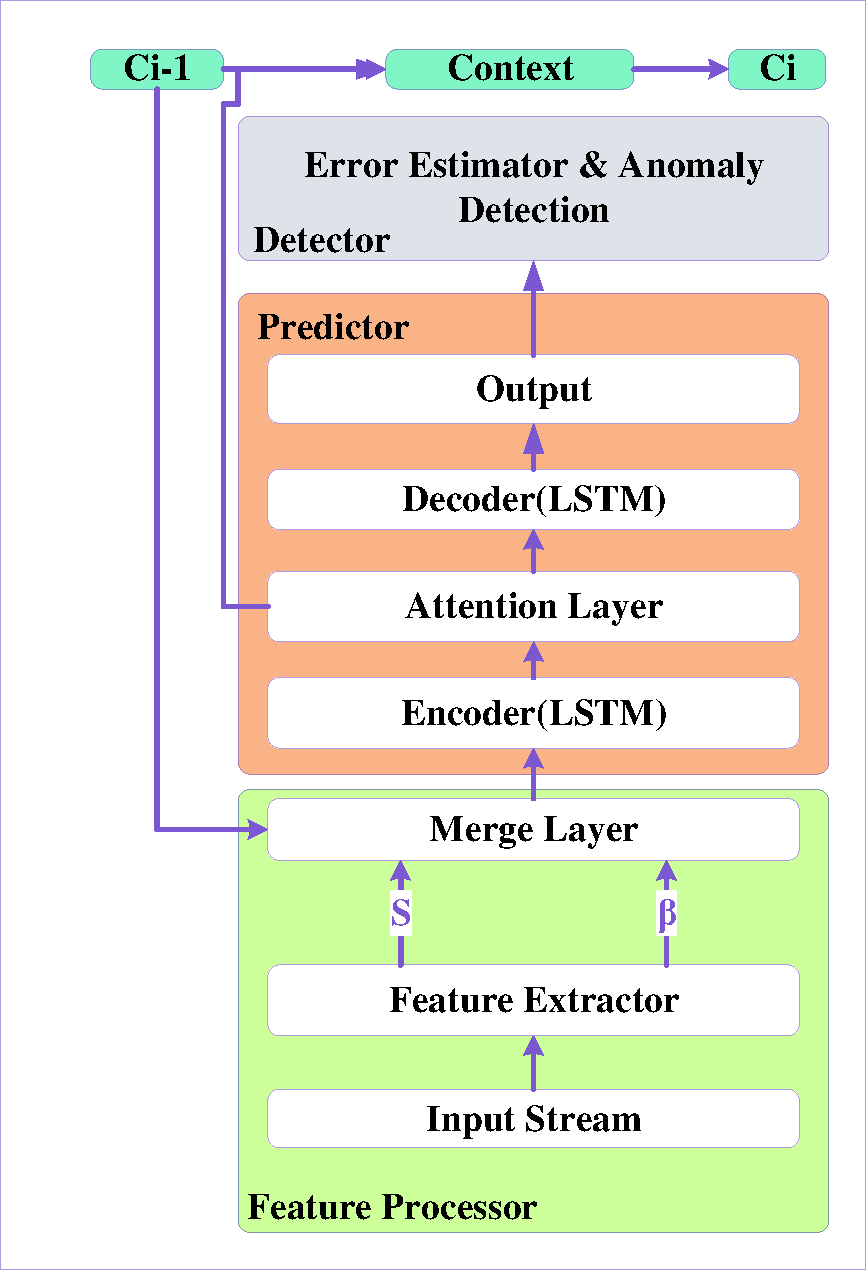
\includegraphics[width=0.4\textwidth, 
	height=9cm]{anomaly-model} 
	\caption{Deep Anomaly Model View with the Feature 
	Processor, Predictor and Detector}
	\label{fig:rnn-model}
\end{figure}

\subsection{Detector}
\label{subsec:detector}
\subsubsection{Error Estimator}
\label{subsec:error-model}
Given $ \bm{x}_i \in \bm{\mathbb{R}} $ which serves as the 
input, the target 
during learning is a shifted version $ \bm{x}_{i+w} \in 
\bm{\mathbb{R}} $ where 
$ \bm{w} $ is the lookahead window. Therefore, the goal is to 
replicate the 
sequence at the output by creating $ \bm{x}' \in 
\bm{\mathbb{R}}$. Hence, the 
perfect result is when $\bm{x}_k  \equiv \bm{x}'_k $, but 
this is hardly 
feasible because of the high randomness caused by interrupts 
and other events 
in the traces. Hence, when we have $ \bm{f}:\bm{x}\longmapsto 
\bm{x}' $ given $ 
\bm{x} $ as the ground truths, the deviation $ \bm{d} = 
|\bm{x} - \bm{x}'|$ is the difference between the ground 
truth and the 
predicted value for the 
given sequence. This deviation becomes the prediction error 
values which we 
process further to decide if an anomaly has occurred or not. 
Our framework is a
\emph{multi-input, multi-output} (MIMO) architecture. Hence, 
the prediction 
error for 
the categorical output is the \emph{Boolean error} between 
the predicted and 
the truth value. While for the regression output, the 
prediction error is the 
absolute difference between the ground truth and the outcome 
of the prediction.

\subsubsection{Anomaly Detector}
\label{subsec:anomaly-detector}
The deviations ${ \bm{d}_v = \left\lbrace \bm{d}_1, \bm{d}_2, 
\bm{d}_3,...,\bm{d}_{|V_j|} \right\rbrace  }$ from the 
validation dataset 
constitute random variables which we have no knowledge of the 
underlying 
distribution. However, since they are error values, we are 
interested in 
creating an upper bound or threshold to detect anomalies. 
Hence, we 
try to create a threshold value for the prediction errors. 
Because we know the 
sample $\bm{\mu}$ and variance $\bm{\sigma}^2$,  we employ 
the \emph{Bienaymé-Chebyshev} inequality to compute the 
threshold. The 
inequality guarantees that no more than a certain fraction of 
values can be 
more that a certain distance from the $ \bm{\mu} $. The 
inequality is stated 
mathematically in \eqref{eq:chebyshev}.
\begin{equation}
\label{eq:chebyshev}
\bm{P}\left(|\bm{X-\mu}| \geq \bm{\Upsilon} \right) \leq 
\frac{\bm{\sigma}^2}{\bm{\Upsilon}^2}
\end{equation}
Although the inequality computes the absolute bound with the 
assumption of a 
symmetric distribution, we use it in our model because we are 
only 
interested in the range where the prediction error $ \bm{d} - 
\bm{\mu} > 1 $. 
Hence, lack of symmetry will not affect the threshold 
computation. Therefore, 
we interchange $ \bm{\Upsilon} $ in \eqref{eq:chebyshev} with 
$ 
|\bm{d-\mu}|$ to derive \eqref{eq:chebyshev-2} which we 
use to compute the 
decreasing probability for increasing deviation $ 
|\bm{d-\mu}| $ where $ 
\bm{d > \mu} $.
\begin{equation}
\label{eq:chebyshev-2}
\bm{P}\left(\bm{d} > \bm{\mu}\right) = 
\bm{P}\left(|\bm{X-\mu}| \geq 
|\bm{d-\mu}| \right) = 
\frac{\bm{\sigma}^2}{(\bm{d-\mu})^2}
\end{equation}
One of the advantages that this technique provides is that we 
do not have to 
know the other parameters of the underlying probability 
distribution. Also, 
instead of creating a binary threshold of \emph{True} or 
\emph{False} values as 
was the case in \cite{ezeme2019dream}, 
this probability gives us an opportunity to quantize the 
anomaly scores into 
bands per one complete cycle of operation like the safety 
integrity level 
(\textit{SIL}) provided by safety 
standards like 
\textit{IEC 61508} \cite{bell2006introduction}. Our quantized 
levels are called 
\emph{anomaly level probability}, ($\bm{AL_{\rho}}$) and each 
level depends on 
the 
value of the probability from \eqref{eq:chebyshev-2}. As 
\eqref{eq:chebyshev-2} 
measures how the error values are clustered around the mean, 
our framework 
should ideally create a high fidelity predictions 
(reconstruction of the normal 
profile sequence) to ensure that \eqref{eq:chebyshev-2} 
performs optimally and 
reduces false negatives.
\subsection{Networking}
As seen in Fig. \ref{fig:dataflow-model}, the dataflow model 
entails a lot of networking between threads, processes and 
nodes. In all, we implemented the networking framework using 
ZeroMQ \cite{zeromq}. Three 
prominent features of ZeroMQ that endeared us to the library 
are:
\begin{enumerate*}[label={\alph*)},font={\bfseries}]
	\item platform agnosticism.
	\item inherently asynchronous by design.
	\item arbitrary connection and disconnection capability 
	without resetting the network, and this aided our 
	parallelism design.
\end{enumerate*}
Hence, the ports in the dataflow model of Fig. 
\ref{fig:dataflow-model} are all binding to 
ZeroMQ sockets.
\begin{figure*}
	\centering
	\begin{subfigure}{0.5\textwidth}
		\centering
		\includegraphics[scale=0.142,keepaspectratio]{%
			cpu-load-no-network}
		\caption{Non Distributed Anomaly Detection 
		Performance}
		\label{fig:Standlone}
	\end{subfigure}%
	\begin{subfigure}{0.5\textwidth}
		\centering
		\includegraphics[scale=0.142,keepaspectratio]{%
			cpu-load-network}
		\caption{Distributed Anomaly Detection Performance of 
			Nodes}
		\label{fig:distributed}
	\end{subfigure}
	\caption{Comparison of the Number of Completed Anomaly 
		Detection Tasks in Distributed vs Non Distributed 
		Environment}
	\label{fig:comparison-of-performance}
\end{figure*}
\section{Experiments and Results}
\label{sec:experiments/results}
\subsection{Experiments}
\label{subsec:experiments}
We setup an experiment with $ \bm{10} $ nodes that can go on 
and off the network at anytime. The nodes are of diverse 
compute capacities ranging from personal computers to 
Raspberry Pi. Some nodes 
have a continuous stream of tasks while other nodes have 
tasks 
that are emitted intermittently or randomly. In each of the 
devices, we 
select the processes to be monitored and the higher the 
number of processes monitored, the higher the load on the 
CPU. The tasks are mixture of high and low priority segments 
where priority is determined by the latency requirement of 
the task segment. Our experimental objectives are:
\begin{enumerate*}[label={\alph*)},font={\bfseries}]
	\item determine the throughput (task completion time) of 
	tasks in an independent node as the CPU load varies 
	and use 
	that as the baseline. 
	\item determine the throughput of 
	nodes when 
	the nodes in a Wi-Fi form an ad-hoc network and use the 
	offloading algorithm for managing task distribution. 
	\item and we show the accuracy of the deep learning model 
	in capturing the anomalies in the system calls.
\end{enumerate*}
We start the access point node since it provides the 
interface for networking and we then start the devices. For 
the purpose of the simulation, the access point node notifies 
each node to disconnect when $ \bm{2\; \text{million}} $ 
tasks 
have been completed and we show the statistics in Section 
\ref{subsec:results}. The nodes stream data logged from 
many processes (normal and anomalous) of an unmanned area 
vehicle application to imitate individual applications in a 
node.

\begin{figure*}
	\centering
	\begin{subfigure}{0.5\textwidth}
		\centering
		\includegraphics[scale=0.142,keepaspectratio]{%
			regression-prediction-error}
		\caption{Regression Error for \emph{random, delay} 
		and \emph{normal} profile}
		\label{fig:regression-error}
	\end{subfigure}%
	\begin{subfigure}{0.5\textwidth}
		\centering
		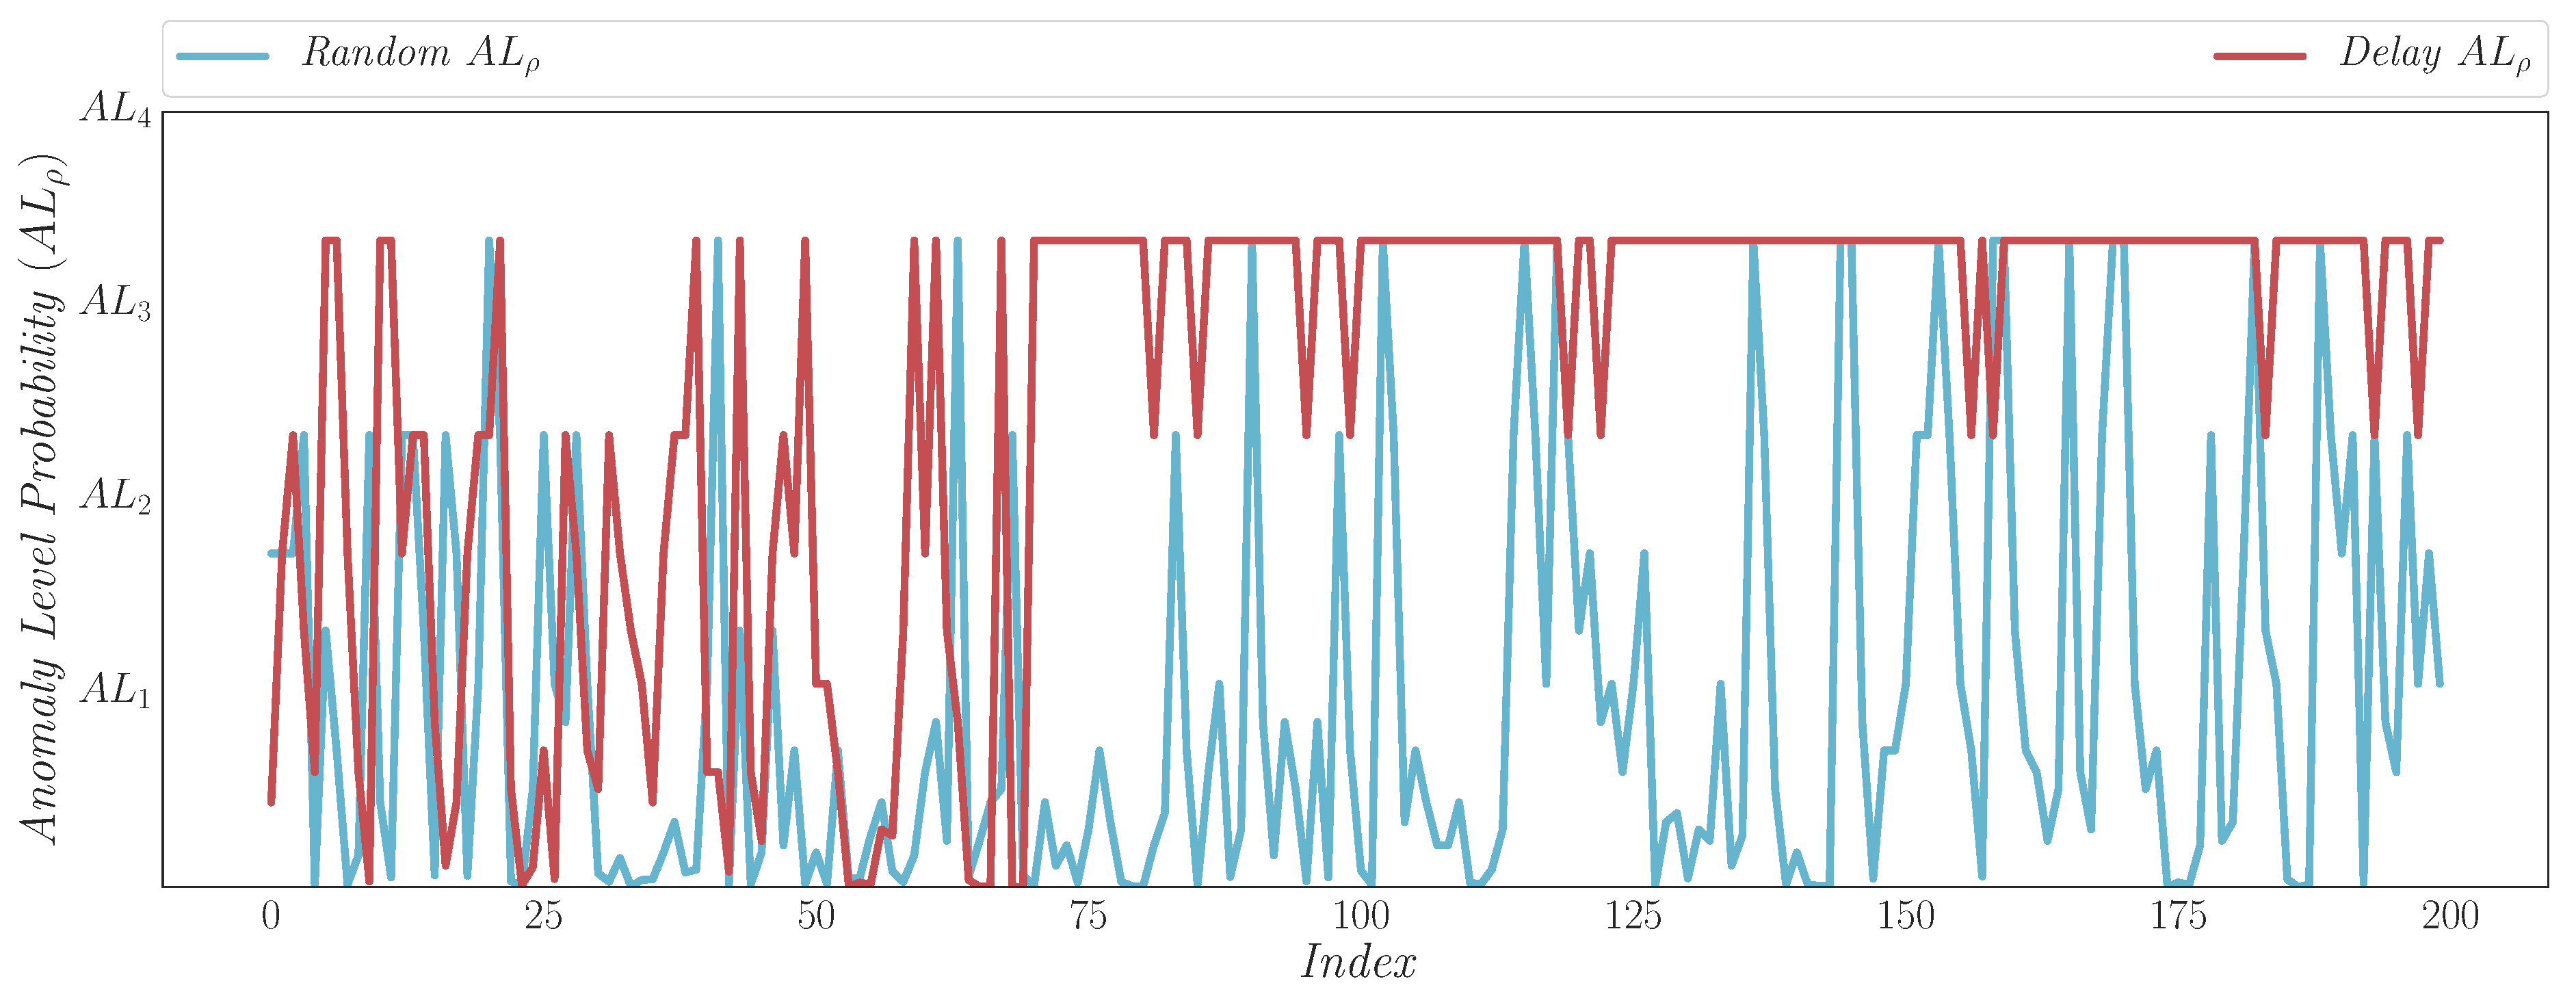
\includegraphics[scale=0.142,keepaspectratio]{regression-anomaly-probabilities}
		\caption{Instruction Cycle Count Anomaly Level 
		Probability, $ 
			\bm{AL_{\rho}} 
			$ }
		\label{fig:ALP}
	\end{subfigure}
	\caption{Regression Error for the \emph{Normal, Random} 
		and  Delay Profile with the $ \bm{AL_{\rho}}$ of the 
		Anomalous Profiles}
	\label{fig:error-ALp}
\end{figure*}

\subsection{Results}
\label{subsec:results}
The data represents three profiles: \emph{normal} (no 
anomalies in the data), \emph{delay} (denial of service kind 
of anomalies) and \emph{random} (information leakage kind of 
anomalies resulting in new kind of sequence ordering). We set 
the tasks to varying degrees of latency requirements up to $ 
\bm{100} $ milliseconds, and we stop the simulation after $ 
\bm{2} $ million tasks have been analyzed. In Fig. 
\ref{fig:comparison-of-performance}, we have plotted the 
percentage of \emph{stale} (anomaly detection tasks that 
could not finish before their timing constraint) for both the 
standalone (where each node works independently) situation 
and the distributed scenario utilizing the offloading 
algorithm under varying CPU load conditions. Comparing Fig. 
\ref{fig:Standlone} and Fig. \ref{fig:distributed}, the 
latter consistently outperforms the former under the various 
CPU load conditions 
except in the \emph{Random} CPU load category. Under the 
\emph{Random} CPU load category, we allowed the CPU load 
utilization to fluctuate between the 
minimum (idle) and maximum (full) value. The result in this 
category under distributed mode is poor as we observed that 
bursty 
traffic by most of the nodes at the same time with short 
latency requirements made it difficult for the scheduling 
algorithm to 
manage the tasks optimally, hence the poor result in this 
category. The high stale tasks in the \emph{Low} and 
\emph{Moderate} CPU load categories in Fig. 
\ref{fig:Standlone} are mostly as a result of 
low capacity nodes which cannot finish tasks within the time 
constraints. Under the \emph{High} CPU load category, because 
some nodes' traffic are bursty in nature (reactive devices), 
the algorithm was able to manage the anomaly tasks by 
utilizing the resources provided by these kind of devices to 
ensure a high throughput. \par 
With respect to the accuracy of the anomaly detector model, 
we 
have shown a snapshot of the prediction error as the tasks 
are executed for the three profiles: \emph{normal, random, 
} and \emph{delay}. As explained in Section 
\ref{subsec:detector}, the 
accuracy of the model hinges on generating low prediction 
error for the \emph{normal} profile and high deviation error 
in any instance of the anomalous sub-sequence that contains 
an anomaly. We work with the replication error since it is an 
\emph{unsupervised} anomaly detection framework. As seen in 
Fig. \ref{fig:regression-error}, the \emph{normal} profile 
generates low regression error (no anomalies) while the 
\emph{delay} and \emph{random} profiles exhibit high 
regression errors when an anomalous sub-sequence task is 
analyzed. Since an increasing value of the error leads to 
reduced chance of the sub-sequence being free of anomalies as 
stated in \eqref{eq:chebyshev-2}, Fig. \ref{fig:ALP} 
displays a snapshot through the \emph{delay} and 
\emph{random} profile with their level of anomalous 
probability. The smaller the value of $ \bm{AL_{\rho}} $ in 
Fig. \ref{fig:ALP}, the greater the severity of the anomaly.

\section{Conclusion}
\label{sec:conclusion}
In this paper, we propose a modular deep learning framework 
and an offloading algorithm that takes advantage of the 
increasing capacity of the edge devices to create a 
distributed anomaly detection framework that brings online 
anomaly detection capability to every node in the network. 
This framework brings improved security to the applications 
or processes in the edge nodes. We test the anomaly framework 
using kernel event streams, and the results confirm the 
ability of the offloading algorithm to manage the anomaly 
tasks with varying timing constraints. The deep 
learning-based anomaly detector also shows a high fidelity 
sequence replication power that ensures that anomalous 
sequences are detected. Our next research direction will be 
on improving the number of completed tasks to ensure that we 
do not miss critical anomalous scenarios.

\section*{Acknowledgements}
This research was funded in part by the Natural Sciences and Engineering Research Council of Canada (NSERC). The first author also acknowledges the support of PTDF Nigeria towards his graduate studies.